%script python
\begin{scontents}[overwrite,write-out=as2024j2exo1.py]
def proba(k) :
	p = 0
	for i in range(k+1) :
		p = p + binomiale(i, 50, 0.065)
	return p
\end{scontents}

Voici la répartition des principaux groupes sanguins des habitants de France.

\begin{Centrage}
\fbox{%
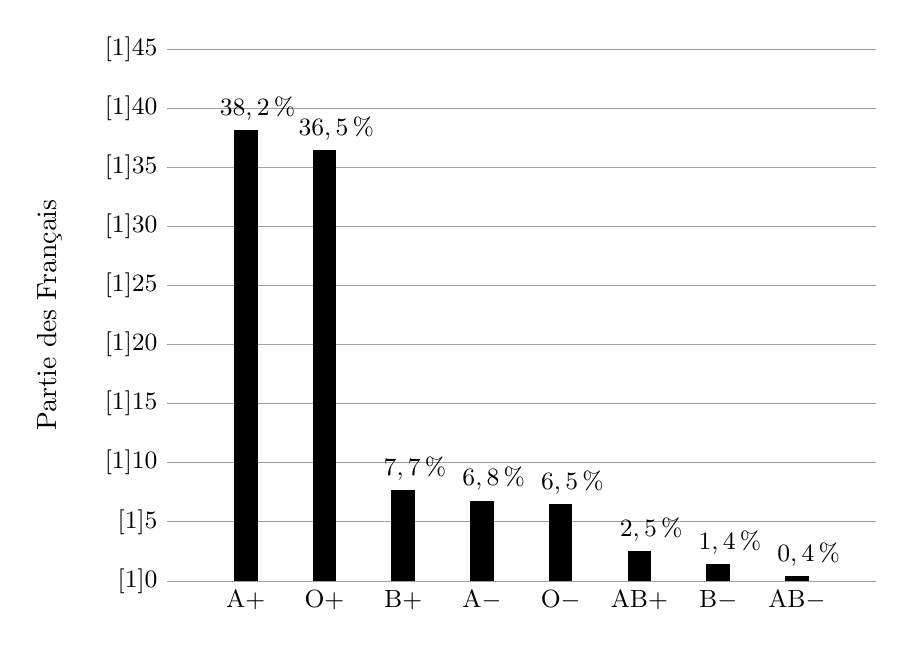
\begin{tikzpicture}[x=1cm,y=0.15cm]
	\foreach \x in {0,5,...,45}{%
		\draw[very thin,gray!75] (-1,\x) node[left,text=black,font=\small] {\pflpcent[1]{\x}}--++ (9,0) ;
	}
	\foreach \gpe [count=\i from 0] in {A+,O+,B+,A$-$,O$-$,AB+,B$-$,AB$-$}{%
		\draw (\i,0) node[below,font=\small] {\gpe} ;
	}
	\fill ({0-0.15},0) rectangle++ (0.30,38.2) node[above,font=\small] {$38,2\,\%$} ;
	\fill ({1-0.15},0) rectangle++ (0.30,36.5) node[above,font=\small] {$36,5\,\%$} ;
	\fill ({2-0.15},0) rectangle++ (0.30,7.7) node[above,font=\small] {$7,7\,\%$} ;
	\fill ({3-0.15},0) rectangle++ (0.30,6.8) node[above,font=\small] {$6,8\,\%$} ;
	\fill ({4-0.15},0) rectangle++ (0.30,6.5) node[above,font=\small] {$6,5\,\%$} ;
	\fill ({5-0.15},0) rectangle++ (0.30,2.5) node[above,font=\small] {$2,5\,\%$} ;
	\fill ({6-0.15},0) rectangle++ (0.30,1.4) node[above,font=\small] {$1,4\,\%$} ;
	\fill ({7-0.15},0) rectangle++ (0.30,0.4) node[above,font=\small] {$0,4\,\%$} ;
	\draw (-2.5,22.5) node[rotate=90] {Partie des Français} ;
\end{tikzpicture}%
}

\medskip

{\footnotesize Source : \url{https://fr.statista.com/statistiques/656036/groupes-sanguins-repartition-rh-france/}.}
\end{Centrage}

\medskip

$A+$, $O+$, $B+$, $A-$, $O-$, $AB+$, $B-$ et $AB-$ sont les différents groupes sanguins combinés aux rhésus.

\smallskip

Par exemple : $A+$ est le groupe sanguin $A$ de rhésus $+$.

\smallskip

Une expérience aléatoire consiste à choisir une personne au hasard dans la population française et à déterminer son groupe sanguin et son rhésus.

\smallskip

Dans l'exercice, on adopte les notations du type :


$A+$ est l'événement \og la personne est de groupe sanguin $A$ et de rhésus $+$ \fg

$A-$ est l'événement \og la personne est de groupe sanguin $A$ et de rhésus $-$ \fg

$A$ est l'événement \og la personne est de groupe sanguin A \fg

\smallskip

Les \textbf{parties} \textbf{1} et \textbf{2} sont indépendantes.

\medskip

\textbf{Partie 1}

\medskip

On note $R\text{h}+$ l'évènement «La personne est de rhésus positif ».

\begin{enumerate}
	\item Justifier que la probabilité que la personne choisie soit de rhésus positif est égale à $0,849$.
	\item Démontrer à l'aide des données de l'énoncé que $P_{R\text{h}+}(A)=0,450$ à $0,001$ près.
	\item Une personne se souvient que son groupe sanguin est $AB$ mais a oublié son rhésus. Quelle est la probabilité que son rhésus soit négatif ? Arrondir le résultat à $0,001$ près.
\end{enumerate}

\medskip

\textbf{Partie 2}

\medskip

Dans cette partie, les résultats seront arrondis à $0,001$ près.

\smallskip

Un donneur universel de sang est une personne de groupe sanguin O et de rhésus négatif. On rappelle que $6,5\,\%$ de la population française est de groupe $0-$.

\begin{enumerate}
	\item On considère 50 personnes choisies au hasard dans la population française et on note $X$ la variable aléatoire qui compte le nombre de donneurs universels.
	\begin{enumerate}
		\item Déterminer la probabilité que 8 personnes soient des donneurs universels.
		
		Justifier votre réponse.
		\item On considère la fonction ci-dessous nommée \texttt{proba} d'argument \texttt{k} écrite en langage \textsf{Python}.
		
		\CodePythonLstFichierAlt*[0.66\linewidth]{center}{as2024j2exo1.py}
		
		Cette fonction utilise la fonction \texttt{binomiale} d'argument \texttt{i}, \texttt{n} et \texttt{p}, créée pour l'occasion, qui renvoie la valeur de la probabilité $P(X=i)$ dans le cas où $X$ suit une loi binomiale de paramètres $n$ et $p$.
		
		Déterminer la valeur numérique renvoyée par la fonction \texttt{proba} lorsqu'on saisit \texttt{proba(8)} dans la console \textsf{Python}. Interpréter ce résultat dans le contexte de l'exercice.

	\end{enumerate}
	\item Quel est le nombre minimal de personnes à choisir au hasard dans la population française pour que la probabilité qu'au moins une des personnes choisies soit donneur universel, soit supérieure à $0,999$.
\end{enumerate}